\documentclass[8pt, letterpaper]{article}
\usepackage[ngerman]{babel}
\usepackage{graphicx}
\usepackage[utf8]{inputenc}
\usepackage{gensymb}
\usepackage{blindtext}
\usepackage{geometry}
\usepackage{fancyhdr}
\usepackage{url}
\usepackage{seqsplit}
\usepackage{hyperref}

\graphicspath{{images/}}
\setlength{\parindent}{0cm}
\bibliographystyle{gerplain}
\geometry{letterpaper, margin=1in}
\pagestyle{fancy}

\lhead{Jakob Kirsch | Paula Lieser}
\rhead{
\includegraphics[width=3cm]{logo}}

% \title{}
% \author{Jakob Kirsch}
% \date{\parbox{\linewidth}{\centering%
%   \today\endgraf\bigskip
%   Fach: \endgraf\medskip
%   Betreuer: \endgraf\medskip
%}}

\begin{document}

% \maketitle
% \newpage
\tableofcontents
% \newpage

\section{Aussage und Zielgruppe}
Unsere Zielgruppe sind Schüler(innen), welche die 10te Klasse abgeschlossen haben, und nicht wissen, welchen weiteren Weg sie einschlagen sollen. Die Werbung soll für unsere Schule mit den Alleinstellungsmerkmalen von GMT und IT werben.

\section{Storyboard}
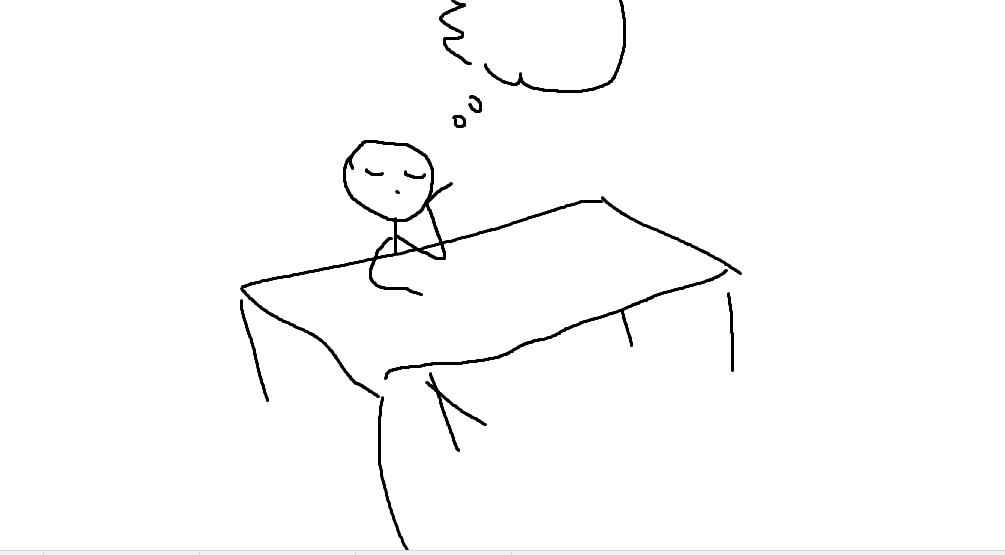
\includegraphics[width=5cm]{scene_1}

Eine Person sitzt an einem Tisch und ist verzweifelt. Das Bild ist leicht drübe. Die Kamera ist in der Aufsicht und geht auf die Person zu. Wir nehmen an, dass viele die Situation kennen, dass man nicht weiß, was man tun soll. In diesem Fall ist die Verzweifelung, was man nach der 10ten Klasse tun soll.

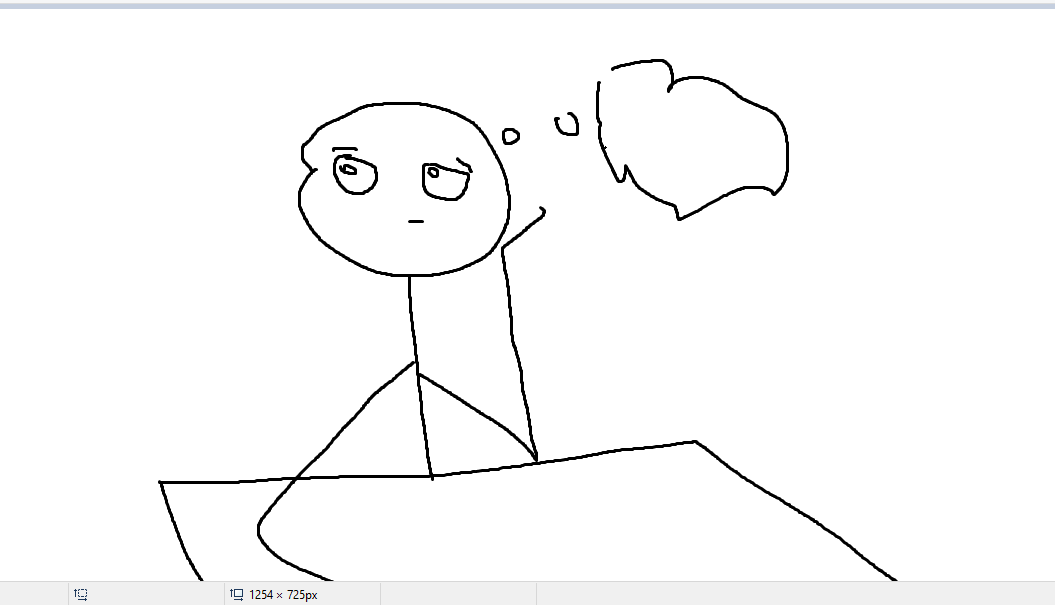
\includegraphics[width=5cm]{scene_2}

Die Kamera nährt sich an die Person an.


\includegraphics[width=5cm]{scene_3}

Eine Stimme spricht zu der Person, welche sich erschreckt und verwundert ist. Die Stimme fragt etwas wie "10 fertig und weißt nicht, was du tun sollst? Hast du an Interesse an Gestaltung und Medientechnik oder Informationstechnik?". Die vorherige Problematik wird angesprochen. Der Zuschauer wird auch gleichzeitig geprimed für die Lösung des Problems, da diese angeteasert wird. Die Farben werden heller und knalliger. Die Kamera stoppt in der neutralen Position. Hier findet man die "attention" des AIDA-Modells.

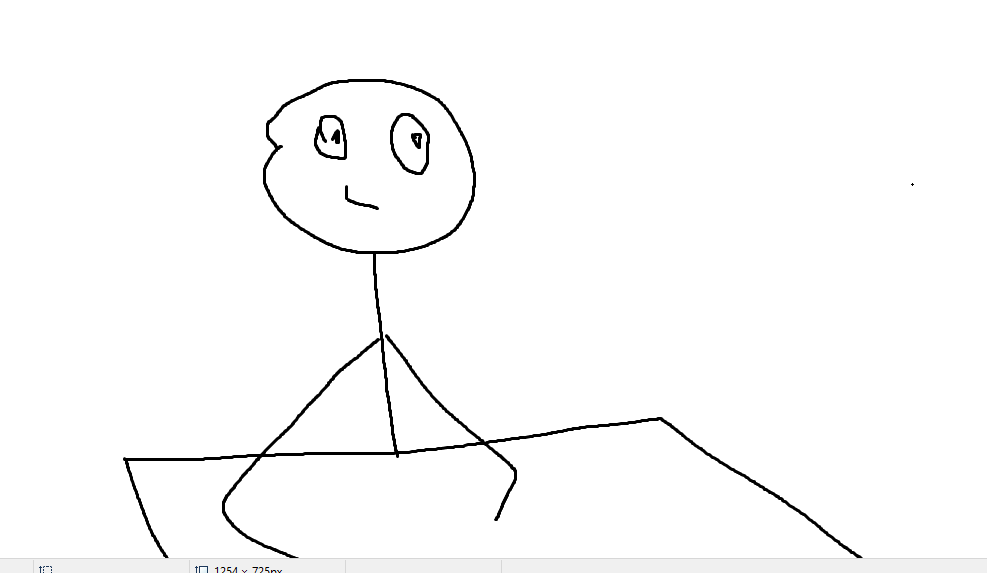
\includegraphics[width=5cm]{scene_4}

Die Person ist positiv überrascht.

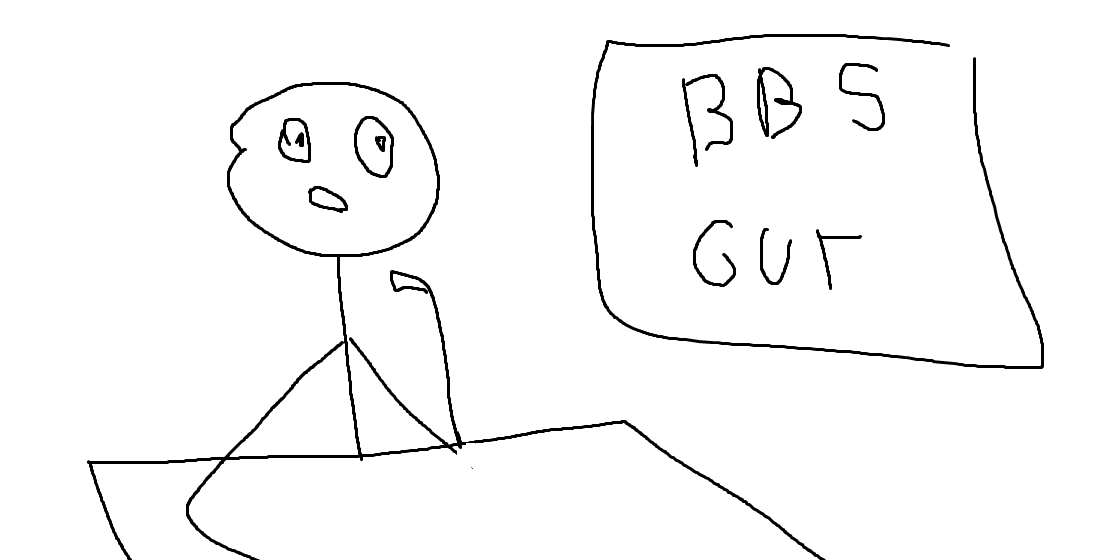
\includegraphics[width=5cm]{scene_5}

Ein Overlay mit dem Schullogo erscheint. Die Stimme sagt etwas wie "Dann komm doch zu uns". Hier wird die vorher angedeutete Lösung präsentiert. Die Person schaut auf das Overlay, um den Fokus komplett auf es zu lenken.


\includegraphics[width=5cm]{scene_6}

Ein weiteres Overlay mit Stichpunkten zu den Wegen von GMT und IT erscheint.


\includegraphics[width=5cm]{scene_7}

Die Person grübelt über das vorher gesagte und ist unentschlossen, wie der Zuschauer es auch sein wird. Hier beginnt die Phase des "interest".

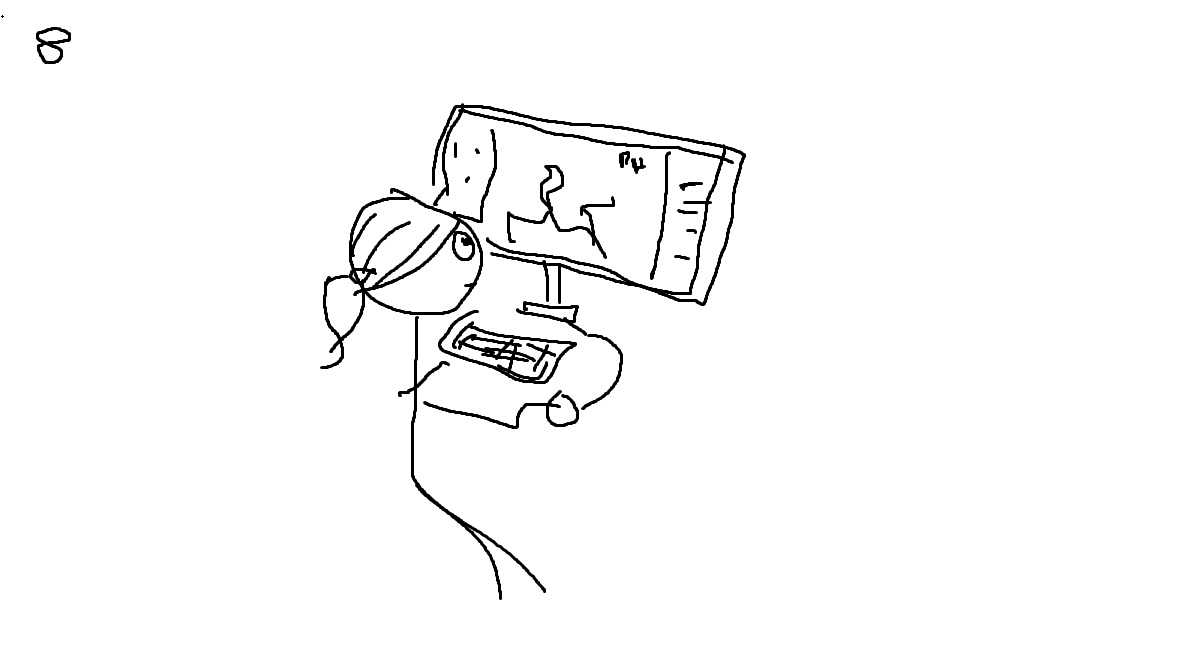
\includegraphics[width=5cm]{scene_8}

Die Kameraperspektive wechselt auf eine Aufsicht einer Person, die an einem Mac arbeitet für GMT. Somit stellen wir den ersten Zweig der Schule vor.

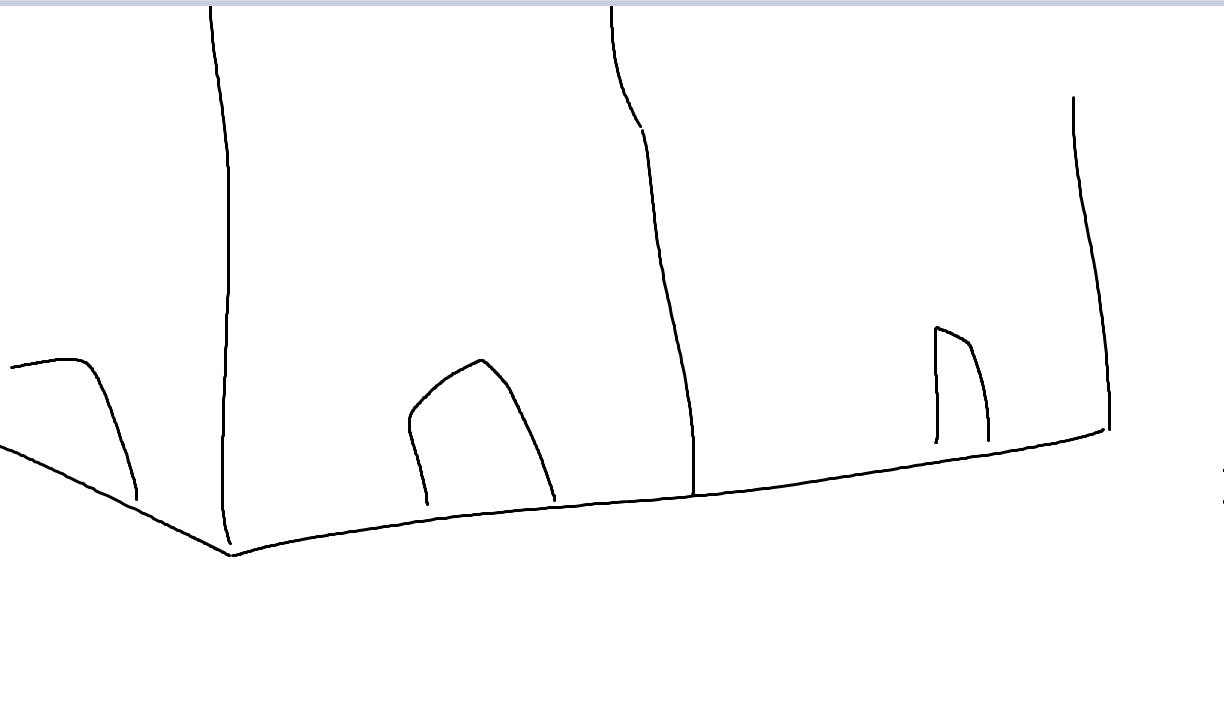
\includegraphics[width=5cm]{scene_9}

Ein slow motion shot der Person mit einer Maus zur Seite und hellen und knalligen Farben zeigt das Arbeiten nochmal im Detail.


\includegraphics[width=5cm]{scene_10}

Die Kameraperspektive wechselt auf eine nahe Kameraperspektive von einem Bildschirm, auf dem Code für einen Arduino zu sehen ist. Dieser ist integraler Bestandteil des IT-Unterrichts in der 11ten Klasse. Die Person wird bewusst ausgelassen, damit der Code zu sehen ist.

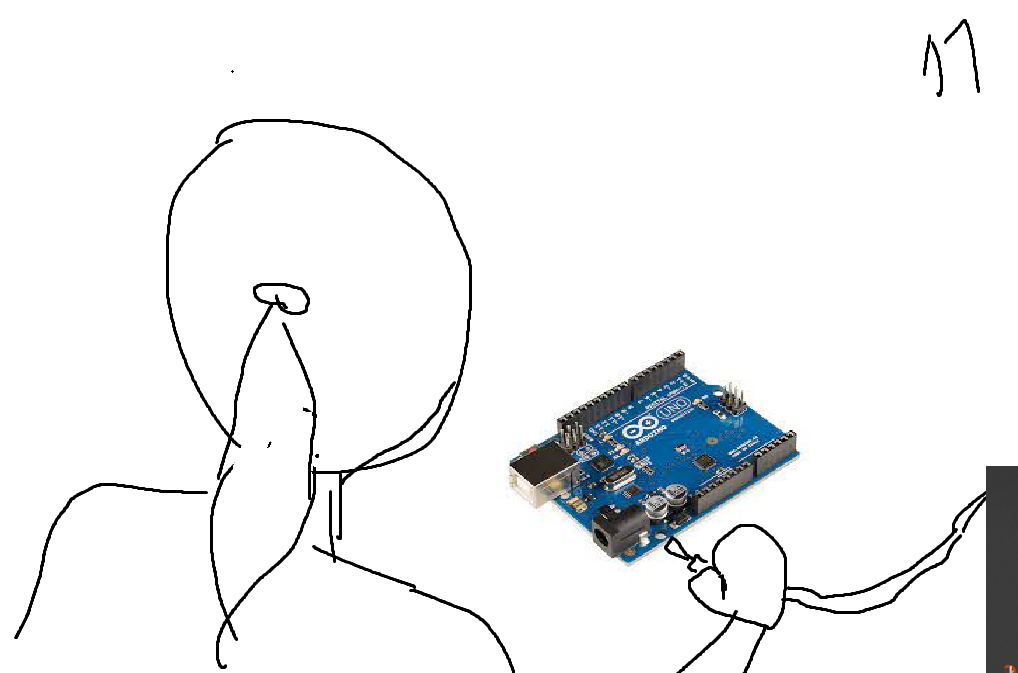
\includegraphics[width=5cm]{scene_11}

Die Person verbindet den Arduino mit einem Kabel in einem overshoulder shot. Auch hier findet wieder eine slow motion statt, welches dem GMT-Teil von vorher ähnelt, was dem Zuschauer etwas Sicherheit suggeriert, da er dieses Muster bereits kennt und somit sich auch besser merken kann.

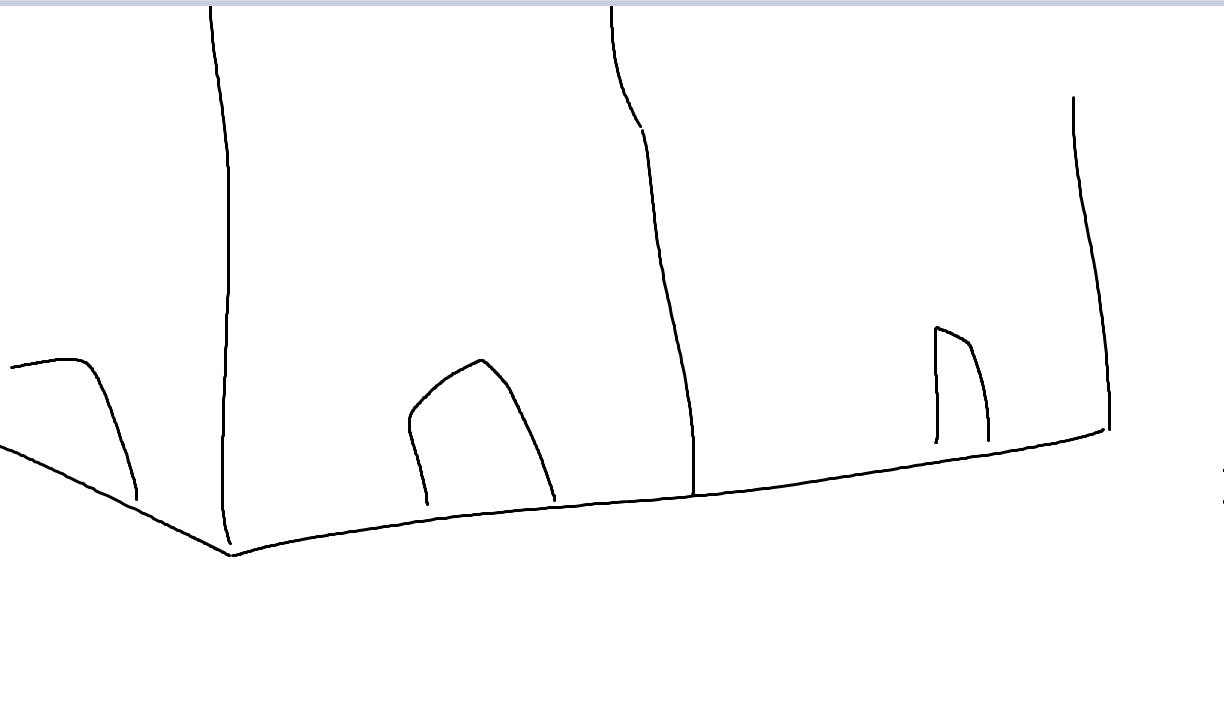
\includegraphics[width=5cm]{scene_12}

Man sieht ein Bild von der Schule, welches auf Augenhöhe aufgenommen wurde. Es enthält knallige und helle Farben. Das vermittelt auch wieder Sicherheit, da man sich die Schule besser vorstellen kann, wenn man ein Bild vor Augen hat.


\includegraphics[width=5cm]{scene_13}

Die Person ist wieder zu sehen. Sie ist glücklich und hat eine Entscheidung getroffen. Sie sagt "Ja, da will ich hin". Das sagt dem Zuschauer schon die "action" und das "desire" vor. Die Stimme gibt noch Informationen zu einem Infoabend, um die "action" so einfach wie möglich zu gestalten.

\section{Klischees und Symbole}
\begin{itemize}
    \item traurige Person, sie wird glücklich und zuversichtlich durch unsere Werbung
    \item Macs für GMT (Design)
    \item Arduino für IT (Mikrokontroller)
\end{itemize}

\section{Figurenanalyse}
Die Hauptfigur unserer Werbung ist zu beginn sehr traurig und verzweifelt, da sie nicht weiß, was sie machen soll. Durch die ihr gebotenen Lösung wird sie glücklich und zuversichtlich. Diese Situation kennen viele Mitglieder unserer potentiellen Zielgruppe. Die Lösung wird als das "Allheilmittel" dargestellt, was dieses Problem magisch verschwinden lässt. Das löst offensichtlich ein gewisses Verlangen aus, wenn man selbst davon betroffen ist. Auch wenn das nicht funktioniert, geben wir immernoch sachliche Argumente (vgl. Szene mit Stichpunkten), warum unsere Schule die genannten Alleinstellungsmerkmale haben.

% \newpage
% \bibliography{refs}

\end{document}
